% =============================================================================
% capitulos/cap1_introducao.tex
%   Cap. 1 -- Introdução e Fundamentação (alvo: 2-3 páginas)
% =============================================================================
\chapter{Introdução}
\label{cap:introducao}


\section{Contexto}
\label{sec:contexto}


A presença de gatos de vida livre (\textit{Felis catus}) em campi universitários é fenômeno documentado em diferentes contextos, com respostas técnicas que buscam conciliar bem-estar animal, saúde pública e conservação da fauna nativa. No Brasil, o paradigma técnico-jurídico adotado para o manejo dessas populações é o protocolo Captura--Esterilização--Devolução (CED), tradução operacional do \textit{Trap--Neuter--Return} (TNR), cuja eficácia em escala continental e em horizonte de longo prazo é descrita em estudos longitudinais clássicos \cite{levy2003longterm,natoli2019italy,kreisler2019orcat} e atualizada em meta-análises recentes \cite{cecchetti2025planning,schiefer2025tnr}. Estudos longitudinais indicam que programas TNR de alta intensidade, espacialmente contíguos, reduzem a densidade populacional e a entrada em abrigos, com ganhos em indicadores de bem-estar \cite{gunther2022reduction,spehar2019backtoschool}. Em campus universitário, o estudo de referência é o programa da \textit{University of Central Florida}, que em 28 anos reduziu sua colônia em mais de 85\% mantendo apenas TNR e adoção \cite{spehar2019backtoschool}; modelo reproduzido em universidades brasileiras, como a Universidade de Brasília (UnB) \cite{junqueira2024evaluation} e a Universidade Federal de Minas Gerais (UFMG) \cite{vecchi2022ethical}, e em outras instituições estrangeiras, como a \textit{University of New South Wales} \cite{passos2025population}.


No Campus 2 da Universidade de São Paulo (USP) em São Carlos, a colônia de aproximadamente 50 gatos distribuídos em 10 pontos de alimentação é manejada pela atividade de extensão AEX Gatos do C2, projeto que reúne docentes, técnicos, funcionários, discentes e voluntários da comunidade externa. A operação segue os princípios do CED, em conformidade com a legislação federal vigente \cite{brasil_lei13426_2017,brasil_lei15046_2024,brasil_decreto12439_2025} e com as Resoluções CFMV nº 1.595/2024 e nº 1.596/2024 \cite{cfmv_resolucao1595_2024,cfmv_resolucao1596_2024}, que padronizam o corte reto da ponta da orelha (\textit{ear-tipping}) como marcador visual primário dos animais esterilizados.


\begin{figure}[!htb]
  \centering
  
\includegraphics[width=0.85\linewidth]{elementos/figuras/cap1-ze-shinji.jpeg}
  \caption[Zé e Shinji, gatos resgatados pelo grupo Gatos do C2.]
  {Zé (à esquerda) e Shinji (à direita), gatos resgatados pelo grupo Gatos do C2 e adotados por voluntário. Zé é proveniente do Campus 2, integrou o protocolo CED e apresenta o corte reto na ponta da orelha (\textit{ear-tipping}); foi removido da colônia por estar muito manso e debilitado. Shinji foi resgatado ainda filhote no Campus 1, em situação de abandono.}
  \label{fig:ze-shinji}
  \fonte{Acervo de Francisco ``Xico'' José, tutor dos animais.}
\end{figure}


\section{O problema}
\label{sec:problema}


A operação cotidiana da AEX Gatos do C2 é hoje sustentada por vigilância humana presencial: voluntários realizam visitas regulares aos pontos de alimentação para reposição de ração, observação clínica e tentativa de manter um cadastro atualizado de indivíduos. Esse modelo enfrenta limitações intrínsecas bem documentadas na literatura. Primeiro, a cobertura temporal é esparsa: as visitas ocorrem em horários compatíveis com a disponibilidade humana, mas a atividade felina é majoritariamente crepuscular e noturna \cite{cove2022capital,herrera2022prey}. Segundo, a identificação individual por inspeção visual é inviável em populações com pelagens parecidas, como sólidos pretos, \textit{tabbys} cinzas e bicolores brancos, gargalo recorrente em estudos de \textit{capture--recapture} urbano \cite{cove2022capital,nakashima2025rest,akbar2025bodypart}. Terceiro, a chegada de novos indivíduos abandonados, evento crítico no campus com impacto direto na dispersão da população, depende hoje da percepção subjetiva dos cuidadores, sem registro objetivo do momento ou do ponto de entrada.


\begin{figure}[!htb]
  \centering
  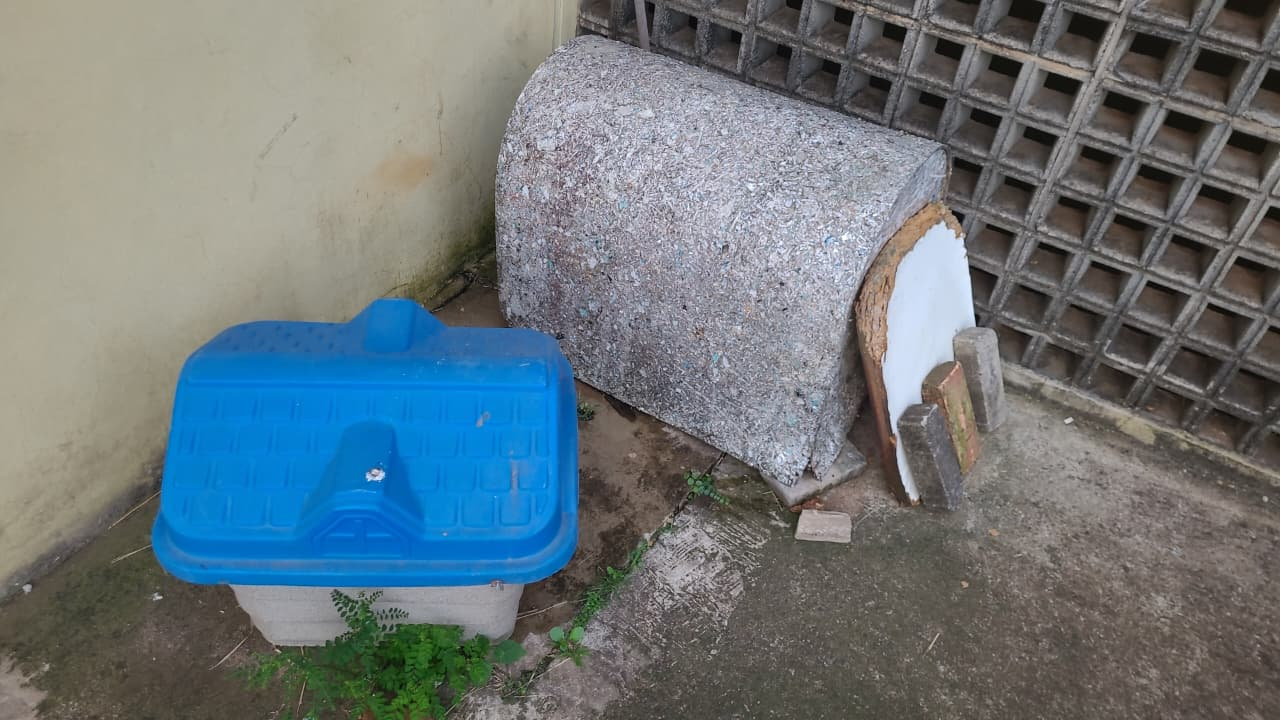
\includegraphics[width=\linewidth]{elementos/figuras/cap1-abrigo.jpeg}
  \caption[Abrigos no ponto de alimentação P03]
  {Ponto de alimentação P03, situado atrás do anfiteatro do Bloco Didático no Campus~2. À esquerda, abrigo plástico; à direita, abrigo de material reciclado. Estruturas como essas integram parte dos dez pontos de alimentação caracterizados no Capítulo~\ref{cap:hardware} e funcionam como referência espacial para o posicionamento das câmeras. A adequação e a melhoria das condições físicas dos pontos de alimentação demandam estudo próprio e não constituem objeto deste trabalho.}
  \label{fig:p03-abrigos}
  \fonte{Acervo do autor, \the\year.}
\end{figure}


O monitoramento sistemático por armadilhas fotográficas (\textit{camera trapping}) é metodologia estabelecida para esse tipo de questão, com três décadas de literatura em ecologia de fauna \cite{bruce2025largescale,cordier2022africa,swanson2015snapshot,cove2022capital}. Câmeras com sensor Passive Infrared (sensor infravermelho passivo) PIR registram presença sem perturbação humana, permitindo estimar riqueza, ocupação, padrões temporais de atividade e, com identificação individual, densidade populacional. A barreira histórica é o volume de imagens: projetos de escala média geram dezenas a centenas de milhares de capturas que excedem a capacidade humana de classificação \cite{norouzzadeh2018automatically,bruce2025largescale}. A aplicação de aprendizado profundo a \textit{camera trapping} atenuou esse gargalo: \citeonline{norouzzadeh2018automatically} demonstraram automação de 99,3\% das classificações do \textit{Snapshot Serengeti} com acurácia equivalente à humana, e o ecossistema atual MegaDetector com PyTorch-Wildlife \cite{hernandez2024pytorchwildlife,microsoft_cameratraps_repo} entrega detecção genérica de animais com licença permissiva e modelos prontos para domínios novos.


A lacuna que motiva este trabalho é específica e atual: não há, na literatura publicada, sistema integrado de monitoramento por visão computacional voltado a colônias de gatos comunitários em campus universitário brasileiro, com o trinômio (i)~detecção robusta a domínios não vistos, (ii)~reidentificação individual (re-ID) capaz de operar em \textit{open-set}, isto é, reconhecer indivíduos novos não cadastrados, e (iii)~validação humana \emph{no laço} para apoio à decisão dos cuidadores. O trabalho metodologicamente mais próximo é o de \citeonline{akbar2025bodypart}, que aplica re-ID por partes do corpo (face, flanco, cauda) a gatos ferais australianos em vegetação natural. O cenário urbano de campus, com diversidade de pelagem e infraestrutura cooperativa de cuidadores, segue pouco abordado na literatura.


\section{Objetivos}
\label{sec:objetivos}


\subsection*{Objetivo geral}


Estudar e conceber um sistema de monitoramento e apoio ao manejo, baseado em visão computacional, para a colônia de gatos comunitários do Campus 2 da USP São Carlos, integrando captura local de imagens, processamento por modelos pré-treinados com adaptação ao domínio e identificação individual com validação humana, em conformidade com o protocolo CED e com a legislação brasileira vigente.


\subsection*{Objetivos específicos}


\begin{enumerate}
  \item[\textbf{O1.}] Caracterizar operacionalmente os 10 pontos de alimentação do Campus 2 quanto a energia, conectividade, fluxo de pessoas e fluxo de animais, gerando os requisitos de hardware.
  \item[\textbf{O2.}] Comparar arquiteturas candidatas de aquisição de imagem (IPCAM, ESP32-CAM e Raspberry Pi com NPU) segundo os critérios de viabilidade, custo total de propriedade e adequação ao campus.
  \item[\textbf{O3.}] Conceber o \textit{pipeline} de visão computacional em quatro fases (ingestão, detecção, classificação e reidentificação), reutilizando modelos abertos de domínio público (MegaDetector v6, CatFLW, PetFace, WildlifeReID-10k) com adaptação local.
  \item[\textbf{O4.}] Definir o protocolo metodológico de avaliação, com escolha de \textit{datasets} de validação, métricas (mAP, F\textsubscript{1}, Rank-$k$) e desenho experimental para falhas previsíveis (oclusão, baixa luminosidade, indivíduos novos).
  \item[\textbf{O5.}] Entregar as bases técnicas e documentais que viabilizem a continuidade do projeto em trabalhos futuros.
\end{enumerate}


Este é um projeto de estudo e concepção. A contribuição central é a arquitetura do sistema, a justificativa técnica das escolhas e os artefatos de engenharia que viabilizam a implementação posterior. A implementação plena, a instalação e a validação em campo permanecem como trabalho futuro.


O detalhamento de infraestrutura física no Capítulo~\ref{cap:hardware} não tem como produto um protótipo físico. Serve para derivar parâmetros operacionais e restrições reais (variabilidade geométrica dos pontos, intermitência energética e presença de fauna não-alvo) que a arquitetura de software precisa suportar.


\section{Justificativa}
\label{sec:justificativa}


A justificativa apoia-se em três eixos. O primeiro é o de \textbf{Saúde Única}: gatos comunitários estão associados a questões zoonóticas relevantes no contexto brasileiro, notadamente a esporotricose felina por \textit{Sporothrix brasiliensis}, em expansão epidêmica no sudeste e sul do país \cite{ferreira2026tndrtm,bastos2025sporotrichosis,colombo2024emergence}\footnote{Micose subcutânea profunda transmitida principalmente por arranhaduras e mordeduras de felinos infectados.}, e a toxoplasmose por \textit{Toxoplasma gondii}\footnote{Zoonose cosmopolita que tem os felídeos como únicos hospedeiros definitivos.}, com seroprevalência documentada em colônias universitárias brasileiras \cite{kmetiuk2021toxoplasma,higa2010toxoplasma}. O monitoramento contínuo e individualizado fornece subsídios para vigilância sanitária integrada \cite{ferroglio2024integrated} e para a tomada de decisão clínica por médicos veterinários \cite{santiago2025sporothrix}.


O segundo eixo é o de \textbf{conservação}: a predação por gatos sobre fauna nativa é problema documentado globalmente \cite{loss2013impact,li2021china}, com revisão específica brasileira recente \cite{goncalves2025wildcat}. Estimar e mapear a pressão de predação no campus exige individualização dos animais, viabilizada pela re-ID em escala.


O terceiro eixo é o da \textbf{lacuna técnica nacional}: enquanto a Europa dispõe da pilha DeepFaune \cite{rigoudy2023deepfaune} e os Estados Unidos da plataforma \textit{Wildlife Insights} com SpeciesNet \cite{wildlifeinsights,google_speciesnet_blog}, não há pilha pública brasileira de monitoramento por visão computacional para fauna sinantrópica\footnote{Espécies silvestres ou asselvajadas que se adaptaram a viver e a se reproduzir em ambientes urbanos, em interação direta com assentamentos humanos.} nem, em particular, para gatos comunitários. Este trabalho contribui para fechar essa lacuna, propondo arquitetura aberta e replicável.


A escolha por reuso de modelos pré-treinados, em vez de treinamento do zero, apoia-se na literatura: detectores generalistas treinados em centenas de \textit{datasets}, como o MegaDetector, generalizam melhor para regiões geográficas não vistas do que classificadores multiespécie treinados localmente \cite{schneider2018avss,velez2022choosing}. O \textit{pipeline} proposto, com detecção genérica seguida de classificação local e de re-ID individual, replica o padrão de engenharia recomendado por \citeonline{mulero2025addressing}, que obteve F\textsubscript{1} de 96,2\% sobre 1,3 milhão de imagens em 24 espécies de mamíferos com poucos milhares de exemplos locais. O módulo de re-ID combina o método de \citeonline{akbar2025bodypart}, com abordagem \textit{part-based} para gatos ferais, com a verificação face a face habilitada pelo \textit{dataset} PetFace \cite{shinoda2024petface}, o maior público para identificação individual em \textit{pets}, com 257 mil indivíduos. A validação cruzada do sistema utiliza o \textit{benchmark} WildlifeReID-10k \cite{adam2024wildlifereid10k} como referência externa, alinhada à competição AnimalCLEF \cite{animalclef2026}.


\section{Organização do trabalho}
\label{sec:organizacao}


O restante desta monografia está organizado em cinco capítulos. O Capítulo~\ref{cap:hardware} trata da aquisição de imagem em campo e abrange a caracterização dos 10 pontos do Campus 2, a análise das arquiteturas candidatas de energia e conectividade e a decisão arquitetural recomendada. O Capítulo~\ref{cap:pipeline} descreve como os dados brutos das câmeras são transformados em registros individuais auditáveis por meio de quatro fases (ingestão, detecção, classificação e reidentificação), fundamentadas em modelos abertos. O Capítulo~\ref{cap:metodologia} detalha os \textit{datasets} de validação, as métricas, o desenho experimental e o tratamento de falhas previsíveis. O Capítulo~\ref{cap:resultados} apresenta os resultados da experimentação do \textit{pipeline} e a avaliação dos modelos. O Capítulo~\ref{cap:conclusao} consolida as contribuições, discute as condições de contorno e indica os trabalhos futuros, com ênfase na continuidade operacional.


Os Apêndices reúnem materiais adicionais ao projeto.
